\section{Diseño del Datawarehouse}
\subsection{Arquitectura BI}
La arquitectura de BI que implementamos para el proyecto sigue un esquema en capas basado en un proceso ETL (Extracción, Transformación y Carga), que permite consolidar y organizar datos provenientes de distintas fuentes operacionales.
\begin{itemize}
    \item {\bfseries Fuentes de datos}
    \begin{itemize}
        \item Una base de datos NoSQL (MongoDB Atlas) que almacena registros detallados y sin procesar de las actividades de los usuarios, recolectados tanto desde las pulseras inteligentes como desde la interacción con la aplicación móvil.
        \item Una base de datos relacional SQL (Supabase, basada en PostgreSQL) que gestiona información administrativa y transaccional, incluyendo datos de usuarios, planes, suscripciones y pagos.
    \end{itemize}
\item{\bfseries Proceso ETL} \par
Los datos se extraen de estas fuentes heterogéneas, luego se transforman para adecuarlos a las reglas del modelo dimensional definido, asegurando la calidad, coherencia y adecuación para análisis posteriores. Finalmente, los datos transformados se cargan en el Data Warehouse central, implementado sobre PostgreSQL en Supabase.
\item{\bfseries Uso posterior} \par
El Data Warehouse alimenta herramientas de visualización y reportes, facilitando la generación de dashboards con indicadores clave para el monitoreo y la toma de decisiones estratégicas del negocio.
\end{itemize}
\subsection{Motor seleccionado}
Para el Data Warehouse hemos elegido PostgreSQL, administrado mediante Supabase, debido a su combinación de robustez, escalabilidad y compatibilidad con operaciones analíticas complejas. Además, su integración con modernas herramientas de BI facilita la elaboración de reportes e informes detallados.




\subsection{Modelado de datos}
El diseño del Data Warehouse se basa en un esquema de modelo en {\bfseries estrella múltiple}, que combina varias tablas de hechos con sus correspondientes tablas de dimensiones
\begin{itemize}
    \item {\bfseries Tablas de hechos} \par
    \begin{itemize}
        \item \texttt{\bfseries hechos\_pagos}, que registra las transacciones relacionadas con la compra de planes y sus características cuantitativas.
        \item \texttt{\bfseries hechos\_actividad}, que almacena los registros de actividades realizadas por los usuarios a lo largo del tiempo.
    \end{itemize}


\item {\bfseries Tablas de dimensiones}\par

\begin{itemize}
    \item \texttt{dim\_usuario}, \texttt{dim\_fecha}, \texttt{dim\_plan}, \texttt{dim\_metodo\_pago}, \texttt{dim\_estado\_pago}, y \texttt{dim\_actividad}, que describen los atributos contextuales para el análisis de los hechos.
\end{itemize}
\end{itemize}
Este enfoque permite realizar análisis multidimensionales eficientes, facilitando el cruce de información desde diferentes perspectivas para obtener insights relevantes sobre el negocio y el comportamiento de los usuarios.

\subsection{Infraestructura usada: Diagramas y Máquinas}
\subsubsection{Diagramas elaborados}
\paragraph{Diagrama de flujo de datos }Representa visualmente el recorrido de la información desde sus fuentes originales (MongoDB y Supabase) hasta su consolidación en el Data Warehouse. Este diagrama facilita la comprensión del pipeline ETL y permite identificar puntos críticos en el proceso.

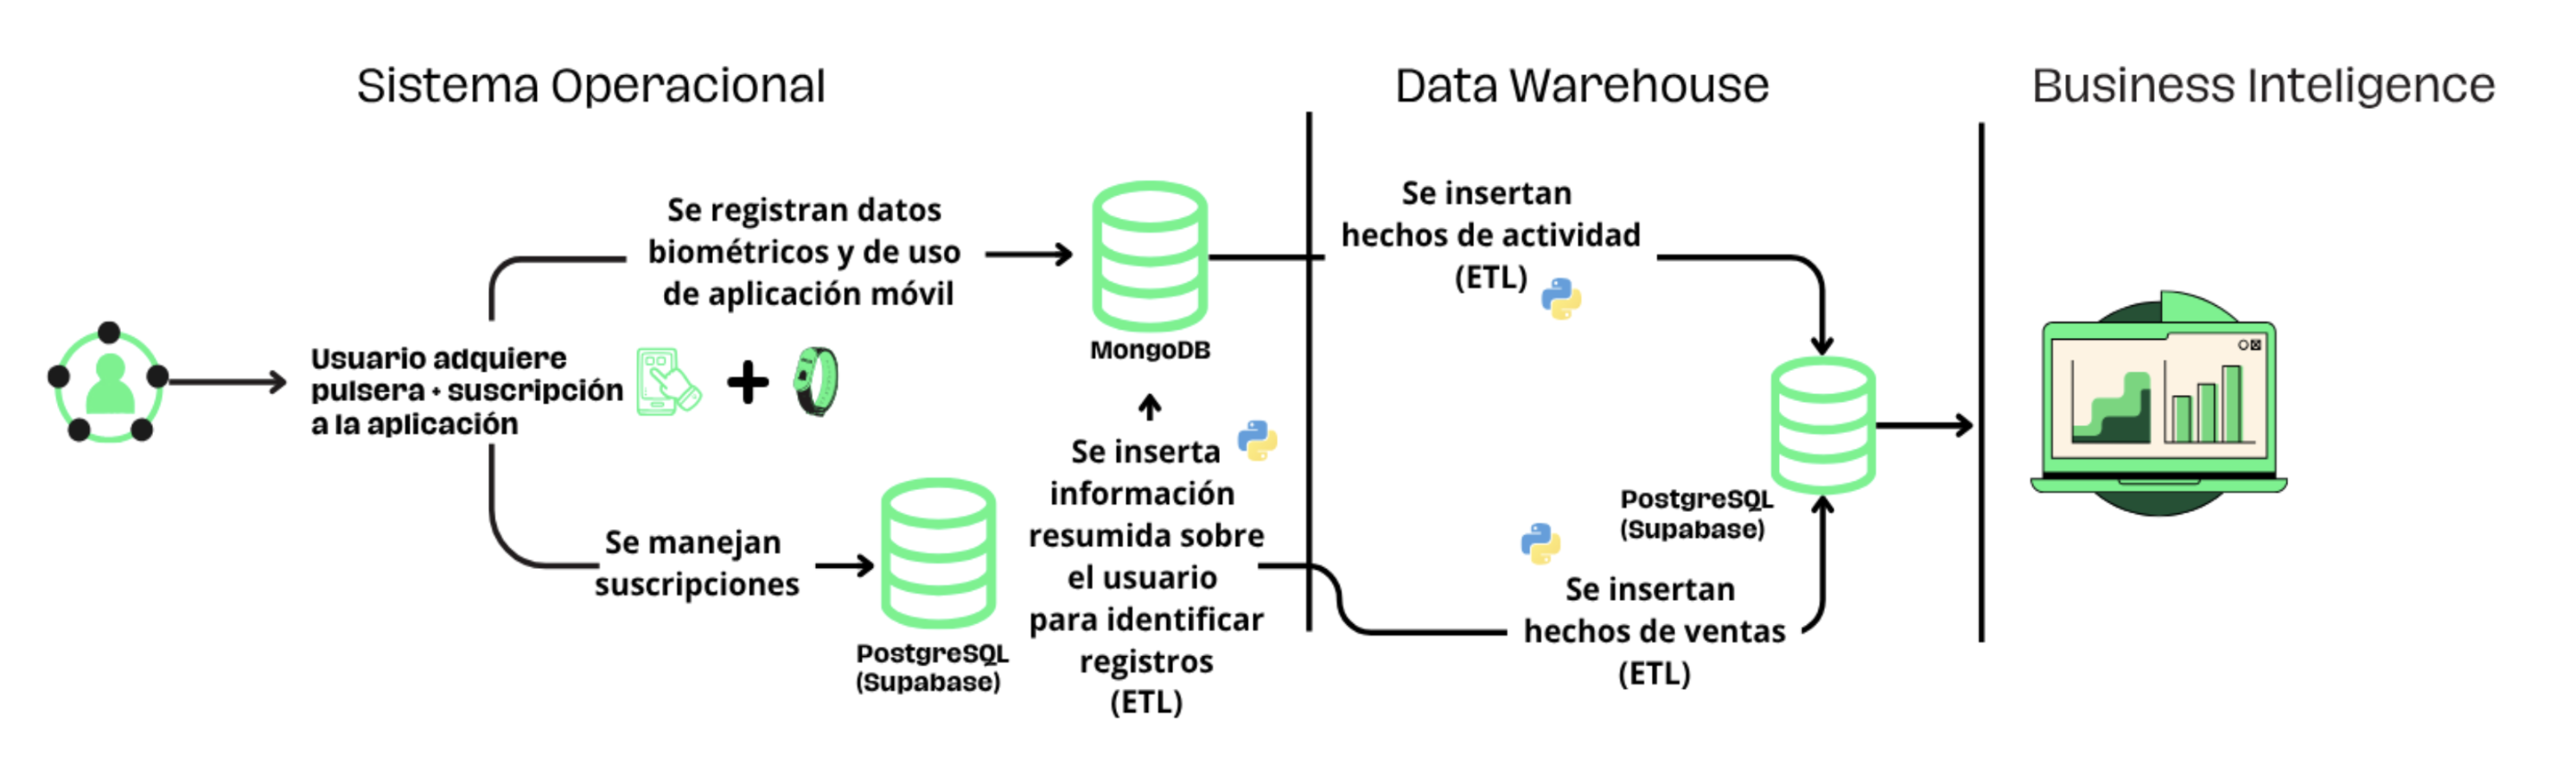
\includegraphics[width=0.95\textwidth]{img/flujo_datos.png}

\paragraph{Diagrama del modelo dimensional} Ilustra el esquema en estrella adoptado, mostrando las relaciones entre las tablas de hechos y las tablas de dimensiones. Este diagrama resulta esencial para entender la estructura del Data Warehouse y permite diseñar consultas analíticas eficientes.

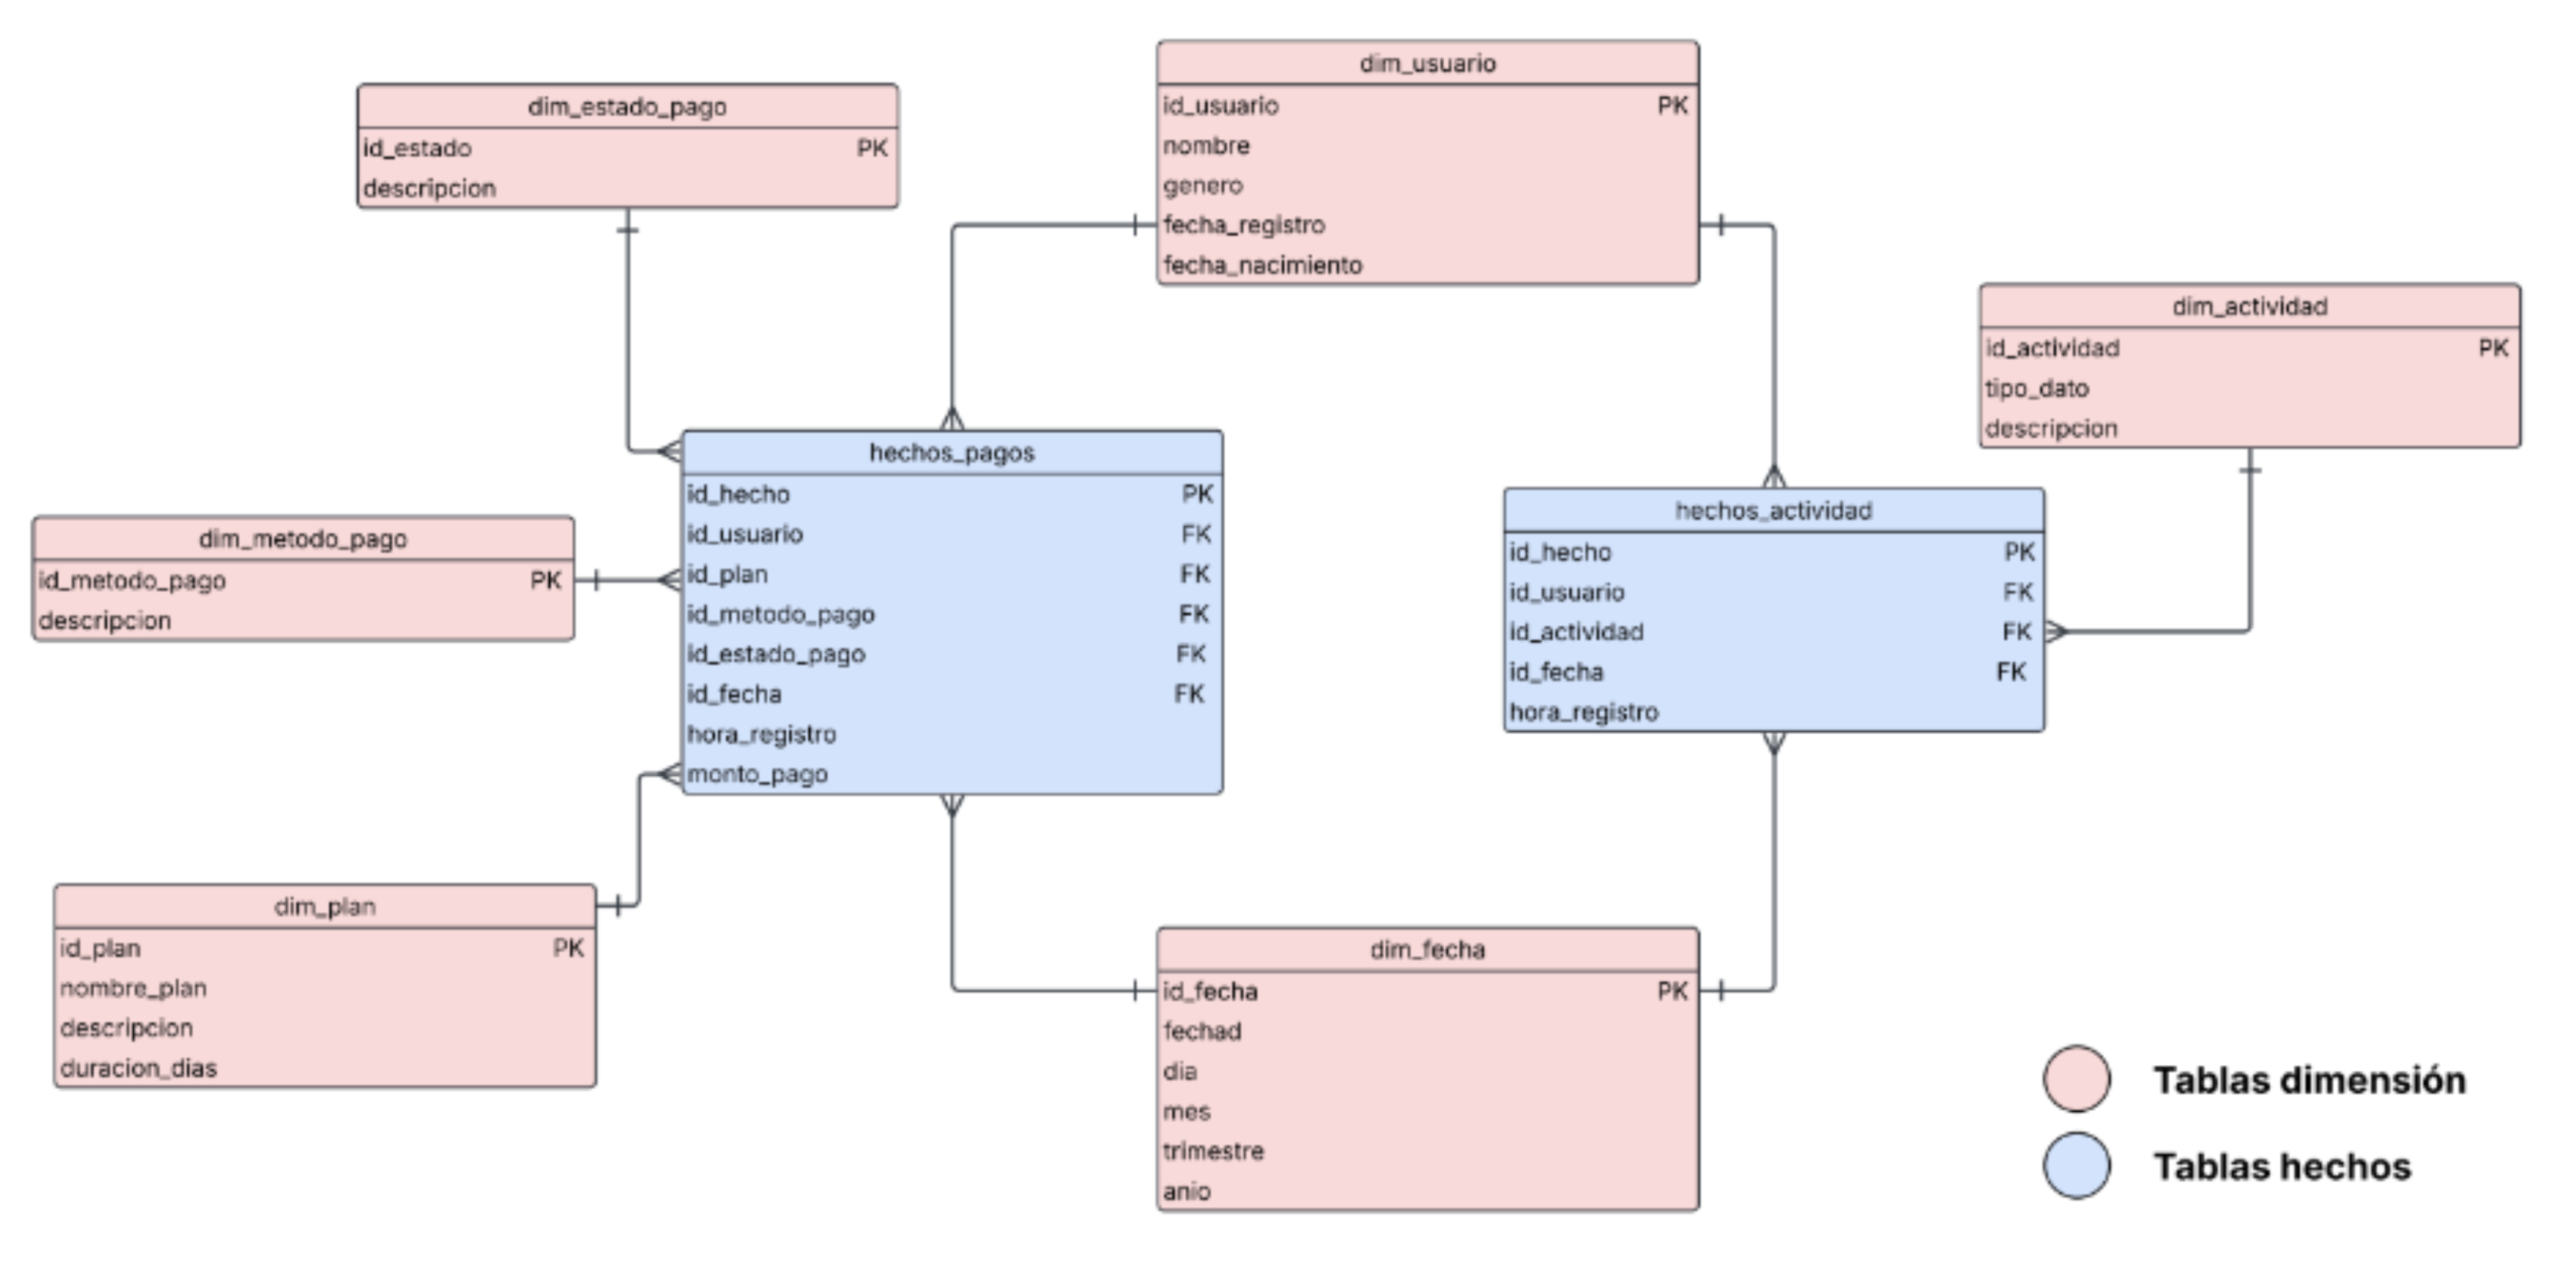
\includegraphics[width=0.9\textwidth]{img/modelo_dimensional.png}

\paragraph{Infraestructura tecnológica y estimación de recursos}
Luego de que las iteraciones pasen el estado de MVP, el volumen de datos provendrá de miles de usuarios que utilizarán simultáneamente las pulseras inteligentes y la aplicación móvil. De esta manera, se tendrá un flujo muy significativo de datos biométricos. La infraestructura deberá estar dimensionada para soportar esta carga sin perder rendimiento ni disponibilidad.
Para ello, seleccionamos servicios gestionados en la nube que sean escalables y balanceados entre las dimensiones de costos y prestaciones:
\begin{itemize}
    \item MongoDB Atlas (NoSQL): Para el almacenamiento de datos biométricos en formato JSON, se estima el uso de un clúster de nivel M20 o superior, que ofrece alrededor de 20 GB de almacenamiento y recursos computacionales suficientes para soportar escritura intensiva, consultas simultáneas y backups automáticos. Este tamaño permite absorber el volumen inicial esperado y crecer conforme aumente la base de usuarios y la frecuencia de recolección de datos.
    \item Supabase (PostgreSQL): Como base para el Data Warehouse y la gestión de datos estructurados de usuarios y suscripciones, se estima un plan con al menos 16 GB de almacenamiento, 4 vCPUs y 8 GB de RAM. Esta capacidad proporciona un rendimiento adecuado para cargas de trabajo analíticas y transaccionales, así como para la ejecución eficiente del pipeline ETL y la consulta de dashboards en tiempo real. De esta manera, la empresa podrá tener flexibilidad para ajustar recursos según la evolución del proyecto.
\end{itemize}


